\chapter{绪论}
\vspace{7pt}

\section{研究背景与目的}
图\ref{fig:test}测试了插图效果:
\begin{figure}[H]
    \centering
    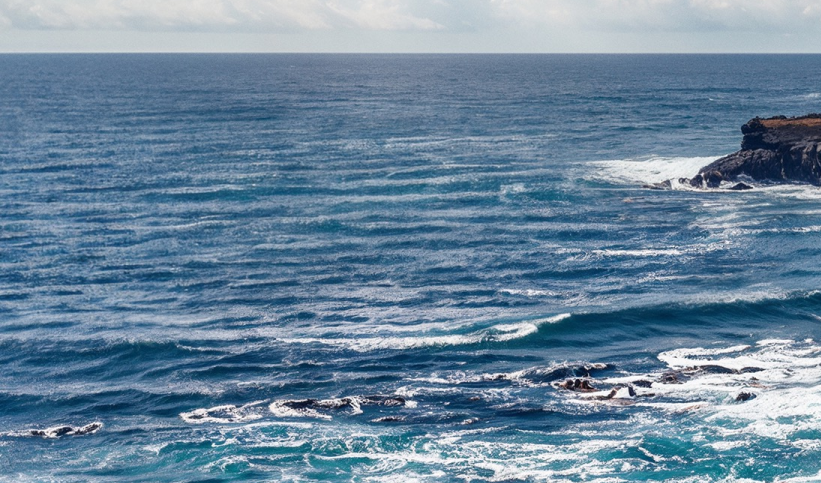
\includegraphics[width=0.75\linewidth]{src//docs//imgs/test.png}
    \caption{图名测试}
    \label{fig:test}
\end{figure}

表\ref{tab:debug_types}测试了插表效果。
\begin{table}[ht]
    \abovetopsep=0pt
    \aboverulesep=0pt
    \belowrulesep=0pt
    \belowbottomsep=0pt
    \begingroup
    \centering
    \caption{表名测试}
    \label{tab:debug_types}
    \fontSimsun\sizeFive
    \newcolumntype{Z}{>{\centering\arraybackslash}X}
    \begin{tabularx}{\textwidth}{Z|Z}
        \toprule
        类型 & 描述 \\
        \hline
        1 & 2 \\
        \hline
        3 & 4 \\
        \hline
        \bottomrule
    \end{tabularx}
    \endgroup
    \vspace{3pt}
\end{table}

\section{研究内容与挑战}

研究面临以下挑战:
\begin{itemize}
  \item TEST1
  \item TEST2
\end{itemize}

本文其余章节安排如下:\hyperref[Related work]{第二章相关工作}综述了XXX